{
{\sffamily Dette afsnit vil præsentere vores resultater fra
eksperimentet, hvor vi har brugt den udvidede metode, til at vurdere
regionerne. Da eksperimentet blev kørt, har vi sat opløsningen på
regionernes approksimation med et gitter for højt, hvilket er resulteret
i, at kørslen ikke er kommet igennem hele vores datasæt.
}

\subsection{Reduceret datasæt}
Kørslen har nået at analysere $608$ malerier, men som vist herunder i
tabel \ref{ud_tabel_fjern_detaljer}, har vi kun $524$ brugbare
resultater, når vi har fjernet de billeder, som ikke er hele malerier.
Dette svarer til en nedgang på $13.82\%$.

\begin{table}[H]
    \centering
    \begin{tabular}{r@{\ \ }p{12em}r|r@{.}l}
            & Analyserede malerier & $608$ & $100$ & $00\%$   \\
        $-$ & Udsnit af malerier   &  $84$ &  $13$ & $82\%$   \\\hline
            & Resultater           & $524$ &  $86$ & $18\%$
    \end{tabular}
    \caption[]{Udregning af brugbare resultater fra udvidet kørsel.}
    \label{ud_tabel_fjern_detaljer}
\end{table}

Dette svarer til $3.65\%$ af de brugbare resultater fra den
naive kørsel. Vores datasæt bliver gennemgået alfabetisk efter
kunstnerens efternavn, så vi har kun resultater fra kunstnere med
efternavn startende med 'A' og 'B'.

At vi kun har et undersæt af malerierne gør, at vi bliver nødt til at se
på hvilke tidsperioder og nationaliteter vi har repræsenteret. Graferne
i figur \ref{ud_year_nation} viser at italienske kunstnere, er kraftigt
overrepræsenteret, og at malerierne primært er fra perioden 1401 --
1650. Dette er ikke overraskende, siden datasættet i forvejen
favoriserer denne type malerier.

\begin{figure}[!h]
    \centering
    \subfloat[Årstal]{
    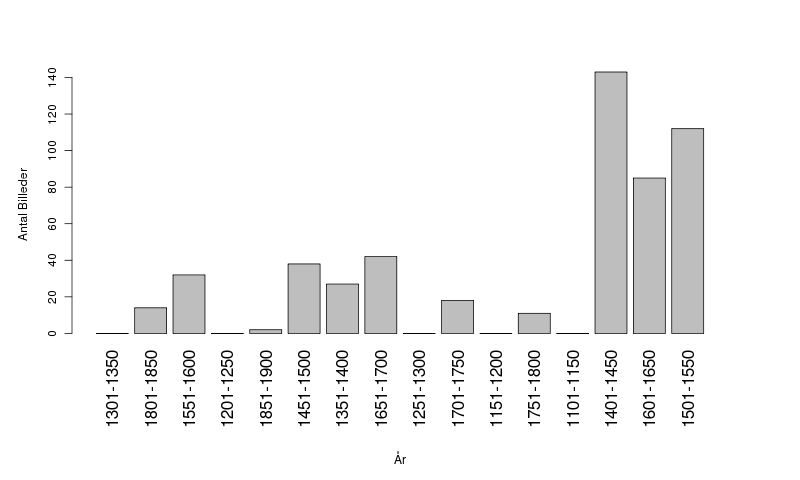
\includegraphics[angle=-90,width=0.42\textwidth]{afsnit/resultater/billeder/year}
        \label{ud_year}}\hspace{1em}
    \subfloat[Nationalitet]{
        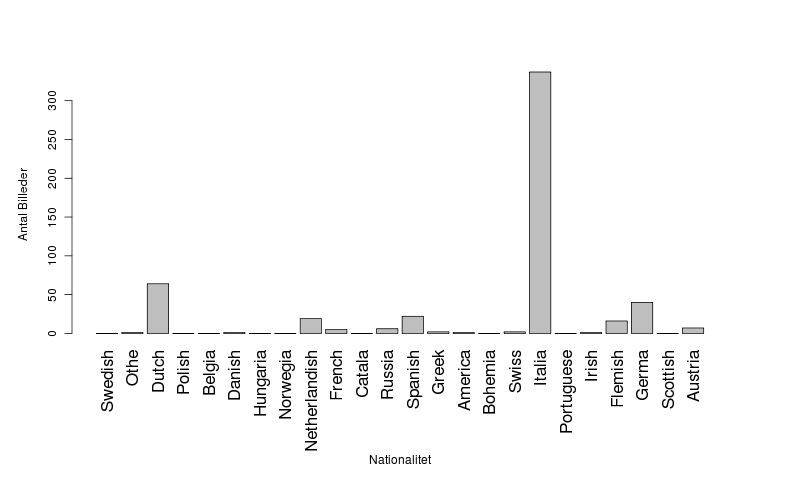
\includegraphics[angle=-90,width=0.42\textwidth]{afsnit/resultater/billeder/nation}
        \label{ud_nation}}
    \caption[]{Maleriernes årstal og nationalitet.}
    \label{ud_year_nation}
\end{figure}

\subsection{Håndtering af systematisk fejl}
Selvom denne analyse også har brugt den fejlbehæftede metode, til
udtrækning af regioner, så sorteres duplikater fra, når vi approksimerer
en region. Vi har gemt farven, som en region er blevet tildelt af
floodfill, og hvis denne farve ikke er at finde i regionens begrænsende
rektangel, betyder det, at regionen er blevet malet over senere. Vi
smider derfor denne region væk.

Den udvidede metode indeholder derfor ingen duplikater, men resultaterne
er ikke direkte sammenlignelige med dem fra den naive kørsel.

\subsection{Resultater}
Udregningen i tabel \ref{ud_tabel_fordeling} redegør for, hvor mange af
de brugbare resultater, der har mindst en region liggende i det gyldne
snit. Vi ser at der i $87.02\%$ af malerierne, er blevet fundet regioner
i det gyldne snit, og vi kan derfor ikke afvise hypotese
\ref{hypo_binaer}.

\begin{table}[H]
    \centering
    \begin{tabular}{r@{\ \ }p{12em}r|r@{.}l}
            & Positive resultater   & $456$ &  $87$ & $02\%$ \\
        $+$ & Negative resultater   &  $68$ &  $12$ & $98\%$ \\\hline
            & Resultater i alt      & $524$ & $100$ & $00\%$
    \end{tabular}
    \caption[]{Et positivt resultat beskriver et maleri hvori der er
    fundet mindst en region i det gyldne snit, ved brug af den udvidede
    vurdering af regioner. Over halvdelen af malerierne har således
    mindst en region i det gyldne snit.}
    \label{ud_tabel_fordeling}
\end{table}

Fordelingen af regioner, over de fire gyldne snit i malerierne, ses i
tabel \ref{ud_tabel_fire_snit}. Intet af de fire snit afviger med
mere end $10\%$ fra et andet, og vi kan således ikke afvise hypotese
\ref{hypo_fire_g_snit}.

\begin{table}[H]
    \centering
    \begin{tabular}{r@{\ \ }p{12em}r|r@{.}l}
            & Regioner i snit 0   &  $405$ &  $22$ & $29\%$ \\
        $+$ & Regioner i snit 1   &  $421$ &  $23$ & $17\%$ \\
        $+$ & Regioner i snit 2   &  $499$ &  $27$ & $46\%$ \\
        $+$ & Regioner i snit 3   &  $492$ &  $27$ & $08\%$ \\\hline
            & Regioner i alt      & $1817$ & $100$ & $00\%$
    \end{tabular}
    \caption[]{Forholdet mellem de interessante regioner fundet i de
    fire gyldne snit ved udvidet vurdering. Antallet af fundne regioner
    i et snit, afviger ikke med mere end $10\%$ fra et andet snit.}
    \label{ud_tabel_fire_snit}
\end{table}


I figur \ref{antal_regioner_vertikale_cut_udvidet} er det samlede antal
fundne regioner, i de 20 vertikale snit, for hele datasættet,
afbilledet. Det ses at der er fundet markant flere regioner, i de to snit som
ligger tættest på miden, og færrest ud i kanterne.

\begin{figure}[h!]
	\begin{center}
		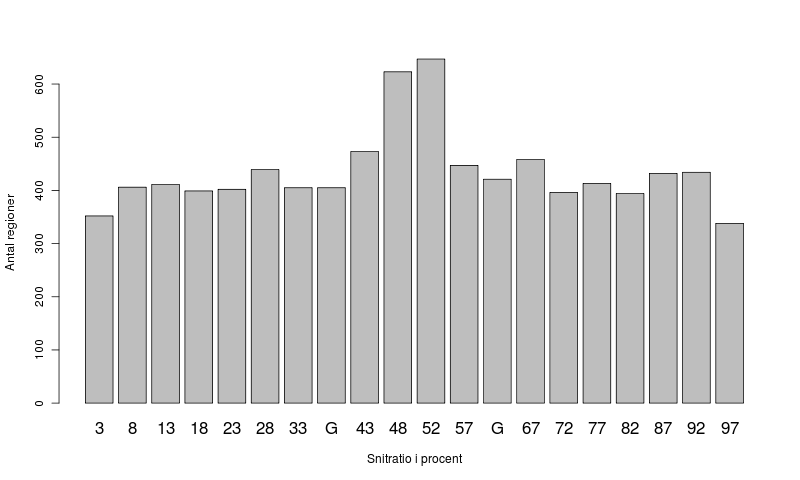
\includegraphics[width=0.9\textwidth]{afsnit/resultater/billeder/cut0cut1eatsperratioU.png}
	\end{center}
	\caption{Antal regioner i hvert af de 20 vertikale snit}
	\label{antal_regioner_vertikale_cut_udvidet}
\end{figure}

I figur \ref{antal_regioner_horisontale_cut_udvidet} er samme afbildning
lavet for det horisontale plan, hvor venstre side af grafen svarer til
toppen af billedet. I denne graf er det snitratioerne $72$ og $82$ som
har flest fundne regioner. Fra snitratio $52$ og ned, falder antal
regioner gradvist. Fra snitratio $52$ og op, svinger antallet af
regioner lidt op og ned. Kanterne er igen klart de laveste i grafen.

\begin{figure}[h!]
	\begin{center}
		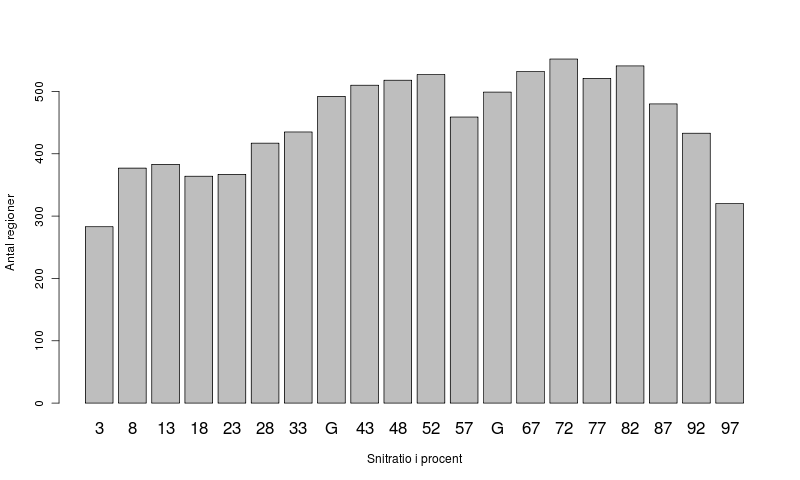
\includegraphics[width=0.9\textwidth]{afsnit/resultater/billeder/cut2cut3eatsperratioU.png}
	\end{center}
    \caption{Antal regioner i hvert af de 20 horisontale snit, hvor
    venstre side af grafen repræsenteree øverste del af malerierne.}
    \label{antal_regioner_horisontale_cut_udvidet}
\end{figure}

Ud fra disse observationer kan vi konkludere at der ikke er flere
regioner i det gyldne snit, end i midten af malerierne, og vi kan derfor
forkaste hypotese \ref{hypo_alle_andre_snit} og \ref{hypo_midten}.

I figur \ref{G_vs_to_trejedele_udvidet}, er de fire gyldne snit, samt
$\frac{2}{3}$ repræsenteret. Det ses at der ikke er nogen entydighed på
hvilken ratio, som er dominerende, og vi kan derfor forkaste hypotese
\ref{hypo_to_tredjedele}.

Figur \ref{G_vs_to_trejedele_udvidet} viser også, at antallet af fundne
regioner i det gyldne snit og
snitratioen $\frac{2}{3}$, ligger meget tæt på hinanden, og den største
forskel ligger ikke på mere end $15\%$. Vi kan derfor ikke afvise
hypotese \ref{hypo_15p}.

\begin{figure}[h!]
	\begin{center}
		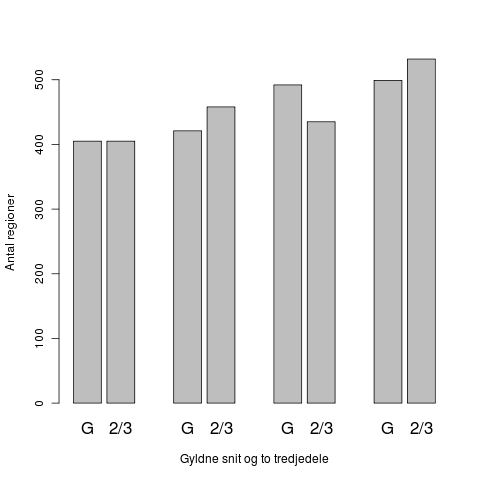
\includegraphics[width=0.6\textwidth]{afsnit/resultater/billeder/G_vs_to_tredjedeleU.png}
	\end{center}
	\caption{Procentvis antal regioner i de fire gyldne snit og deres
    tilhørende $\frac{2}{3}$-snit.}
	\label{G_vs_to_trejedele_udvidet}
\end{figure}

I graferne i figur \ref{udvidet_year},kan man se hvor mange regioner der
er fundet i gennemsnit per billedet i alle tidsperioder. Tidsperioder,
hvor ingen malerier er analyseret, er ikke taget med. Det ses at i
tidsperioden 1401-1450, bliver fundet mange flere en de andre
tidsperioder, og i visse tilfælde doubel så mange, da double så mange
regioner er skrapt støre en $10\%$ afvigelse. Kan vi forkaste hypotese
\ref{hypo_tid}.

\begin{figure}[!h]
	\begin{center}
		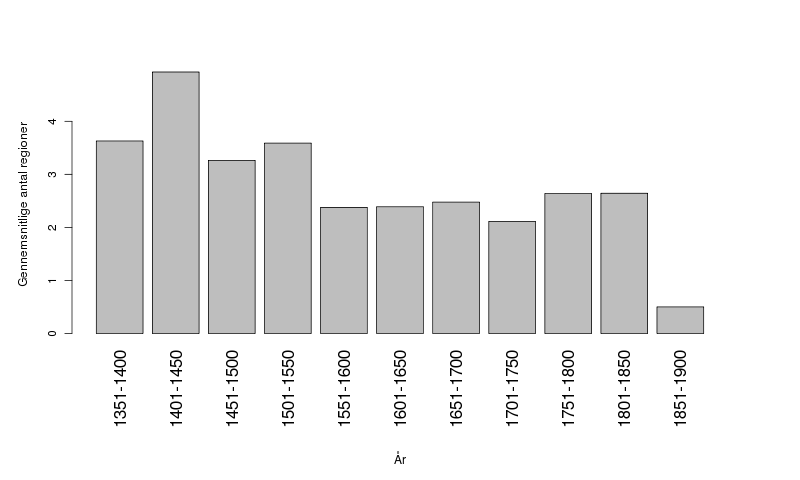
\includegraphics[angle=0,width=0.90\textwidth]{afsnit/resultater/billeder/yearcutU.png}
	\end{center}
	\caption{Graf over antal regioner fundet i hver
       tidsperiode. Hver graf repræsenterer hvert deres snit. Y-aksen er
       det gemmesnitlige antal fundene regioner i snittet.}
	\label{udvidet_year}
\end{figure}

I graferne i figur \ref{udvidet_nation}, ses at det er meget svingene
fra hvilke nationer, billeder med mange regioner i det gyldne snit,
kommer fra. Holland ligger sig lidt foran de andre. Danmark har slet
ikke nogle malerier hvor der er fundet regioner i det gyldne snit. Alle
nationer, hvor analysen ikke har bearbejdet nogle malerier, er sorteret
fra. Da malerier fra Holland har flere end $10\%$ højre gennemsnitlige
fundne regioner, end Danmark og Frankrig, holder hypotese
\ref{hypo_nation} ikke, og kan derfor forkastes.


\begin{figure}[!h]
	\begin{center}
		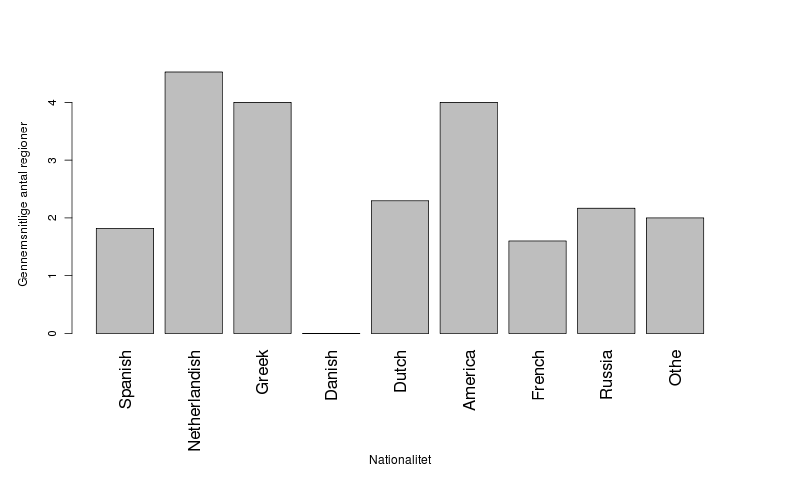
\includegraphics[angle=0,width=0.90\textwidth]{afsnit/resultater/billeder/nationcutU.png}
	\end{center}
	\caption{Graf over antal fundne regioner fundet hver sin
       nationalitet. Hver graf repræsenterer hvert deres snit. Y-aksen
       er det gemmesnitlige antal fundne regioner i snittet.}
	\label{udvidet_nation}
\end{figure}


\begin{table}[!h]
    \centering
    \begin{tabular}{|l|c|c|}
        \hline
            & Afvist & Ikke afvist  \\\hline
        1   &            & \checkmark   \\\hline
        2   &            & \checkmark   \\\hline
        3   & \checkmark$^{\textrm{*}}$ &              \\\hline
        4   & \checkmark &              \\\hline
        5   & \checkmark &    	\\\hline
        6   & \checkmark &              \\\hline
        7   & \checkmark &              \\\hline
        8   & \checkmark &              \\\hline
        9   &            & \checkmark	\\\hline
    \end{tabular}
    \caption[]{Hypoteser i forhold til den udvidede kørsel.
    $^{\textrm{*}}$Jvf. udregning \ref{tabel_real_dimensions}.
    }
    \label{hypoteser_udvidet}
\end{table}

\subsubsection{Antallet af fundne regioner over alle snit}
Analysen har fundet $17,705$ regioner over alle snit i malerierne, med
middelværdi $\mu = 33.79$ og standardafgivelse $\sigma = 18.58$.
Antallet af fundne regioner i malerierne er illustreret i figur
\ref{ud_graf_total_regions}. I figur \ref{ud_qq_total_regions} er vist
et QQ-plot, som viser hvorvidt vores data er normalfordelt. Dette er
tilfældet, hvis punkterne følger diagonalen i grafen. Vi ser, at de
observerede data følger linjen nogenlunde, men har et udsving nederst
til venstre, hvilket antyder at fordelingen er lidt skæv. Vi har i figur
\ref{ud_hist_total_regions} sammenlignet et histogram over de
observerede værdier, med tæthedsfunktionen for normalfordelingen $X \sim
N(\mu = 33.79, \sigma^2 = 345.22)$. De observerede værdier, følger dog
ikke de teoretiske værdier særlig pænt, og kun få steder falder de
teoretiske værdier inden for det observerede interval, hvorfor vi ikke
kan komme frem til et troværdigt konfidensinterval.

Med et større antal fundne regioner, kunne vi meget vel komme tættere på
en normalfordeling, og vi kunne da udtale os mere sikkert, om det
forventede antal fundne regioner i et arbitrært billede.

\begin{figure}[!h]
    \centering
    \subfloat[]{
        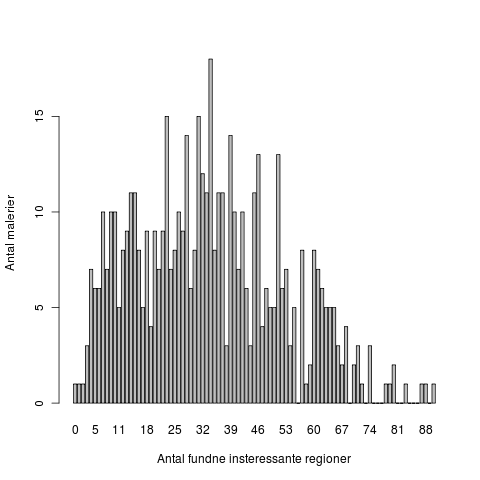
\includegraphics[width=0.49\textwidth]{afsnit/resultater/billeder/exp_totalregions}
        \label{ud_graf_total_regions}
    }
    \subfloat[]{
        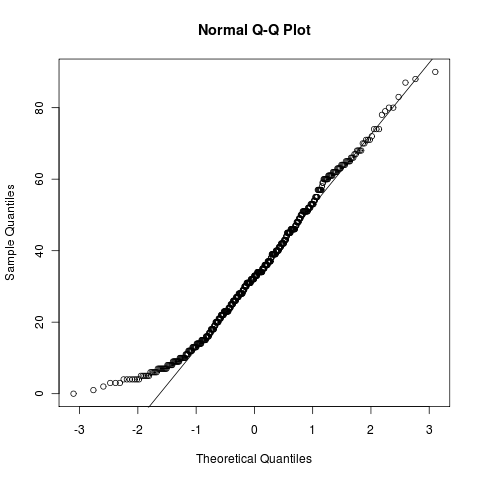
\includegraphics[width=0.49\textwidth]{afsnit/resultater/billeder/qq_exp_totalregions}
        \label{ud_qq_total_regions}
    }\\
    \subfloat[]{
        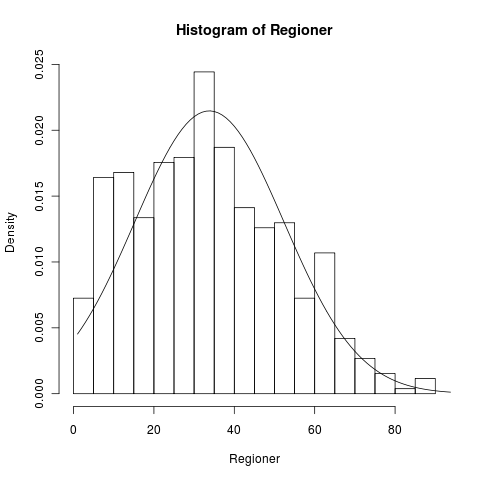
\includegraphics[width=0.62\textwidth]{afsnit/resultater/billeder/hist_exp_totalregions}
        \label{ud_hist_total_regions}
    }
    \caption[]{Fordelingen af fundne regioner på malerier ved udvidet
    vurdering.
    \textbf{\ref{ud_graf_total_regions}:} Fordelingen af de fundne
    regioner.
    \textbf{\ref{ud_qq_total_regions}:} QQ-plot, som viser at vi er tæt
    på at have en normalfordeling med den teoretiske fordeling $X \sim N(\mu,
    \sigma^2)$.
    \textbf{\ref{ud_hist_total_regions}:} Histrogram med
    tæthedsfunktionen for normalfordeling, hvor $\mu = 33.79$ og
    $\sigma^2 = 345.22$.
    }
    \label{ud_total_regions_plots}
\end{figure}

} % Eh eh eh. Nallerne væk!

% vim: set tw=72 spell spelllang=da:
